\section{Protokoll}
% ü ä ß damit jeder editor diese datei als utf8 abspeichern kann

\subsection{Beschreibung}
Das Protokoll von BaseTorrent basiert auf Nachrichtenübermittlung mit \gls{udp} und Datenübermittlung mit \gls{tcp}.\\
Bei Verlust von \gls{udp}-Nachrichten wird nach einer einstellbaren Wartezeit erneut gesendet.\\
Die Suchnachrichten werden gestaffelt versendet, d.h. aus der Liste der \gls{node}s werden der Reihe nach eine gewisse Anzahl an \gls{node}s angeschrieben, um das Netzwerk nicht unnötig zu belasten.

\subsubsection{\texttt{status}-Nachricht}
\label{sec:statusmeldung}
\msgtab{Informiert die bekannten \gls{peer}s aus der eigenen \gls{peerliste}, dass man noch mit dem \gls{btn} verbunden ist.}
{\gls{udp}}
{aktuelle \gls{peerliste}}
{\begin{enumerate}
	\item Prüfe die Liste auf Aktualität 
	\item Sende die eigene aktualisierte \gls{peerliste}
\end{enumerate}}


\subsubsection{\texttt{get}-Nachricht}
\label{proto:get}
\msgtab{\gls{daten}-\gls{btfp}-Anfrage an \gls{peer} X, um Daten von X auf den \gls{bta}-Computer zu kopieren.}
{\gls{udp}}
{\gls{btfp}-\gls{hash}, ein eigener \gls{tcp}-\gls{port}}
{\begin{enumerate} \item Lädt die Daten, wenn sie existieren, über den \gls{tcp}-\gls{port} hoch \end{enumerate}}


\subsubsection{\texttt{store}-Nachricht}
\label{sec:speicheranfrage}
\msgtab{Frage an, wer die eigenen Daten aufnehmen kann.}
{\gls{udp}}
{Part-Hash, Metadaten, \gls{tcp}-\gls{port}, Dateigröße}
{\begin{enumerate}
	\item Prüfe auf Vorhandensein
	\item Prüfe freien Speicherplatz
	\item Wenn beides vorhanden, dann Datei herunterladen
\end{enumerate}}


\subsubsection{\texttt{find}-Nachricht}
\label{sec:dateianfrage}
\msgtab{Anfrage an Peer, ob er Datei x hat.}
{\gls{udp}}
{Liste mit Schlüsselwörtern}
{\begin{enumerate}
	\item Prüfe auf Vorhandensein der Datei.
	\item Wenn Datei vorhanden, dann antwortet mit den Metadaten
\end{enumerate}}


\subsubsection{\texttt{meta}-Nachricht}
\label{sec:metaantwort}
\msgtab{Antwort, ob Peer eine Datei x hat.}
{\gls{udp}}
{Metadaten}
{\begin{enumerate}
	\item Antwortet mit den Metadaten
\end{enumerate}}


\subsubsection{\texttt{listBackups}-Nachricht}
\label{sec:backupanfrage}
\msgtab{Anfrage ob Peer BackUps vom Autor y hat.}
{\gls{udp}}
{Autor}
{\begin{enumerate}
	\item Wenn Datei vorhanden, dann "Meta Antwort"
\end{enumerate}}

\subsubsection{\texttt{deleteBackups}-Nachricht}
\label{sec:backuploeschen}
\msgtab{Löschen von Backups.}
{\gls{udp}}
{\gls{btfp}-\gls{hash}, \gls{Part-Passwort}}
{\begin{enumerate}
	\item Prüfe auf Vorhandensein der Datei.
	\item Prüfe auf Übereinstimmung von Autor und durch \gls{Part-Passwort} entschlüsseltem Autor
	\item Wenn Bedingungen erfüllt, dann Datei löschen
\end{enumerate}}

\subsubsection{\texttt{checkParts}-Nachricht}
\label{sec:redundanzpruefen}
\msgtab{Fragt nach, wie oft ein gewisser Part noch im Netz vorhanden ist.}
{\gls{udp}}
{Liste von Part-Hashes}
{\begin{enumerate}
	\item Prüfe auf Vorhandensein der Datei
	\item Wenn Datei vorhanden, dann "Meta Antwort"
\end{enumerate}}

\newpage

\subsection{Zulässige Nachrichtensequenzen}
Die folgenden Sequenzdiagramme zeigen die zulässigen interessanten Nachrichtensequenzen auf (bei den anderen ist dies trivial):
\begin{figure}[hpt]
	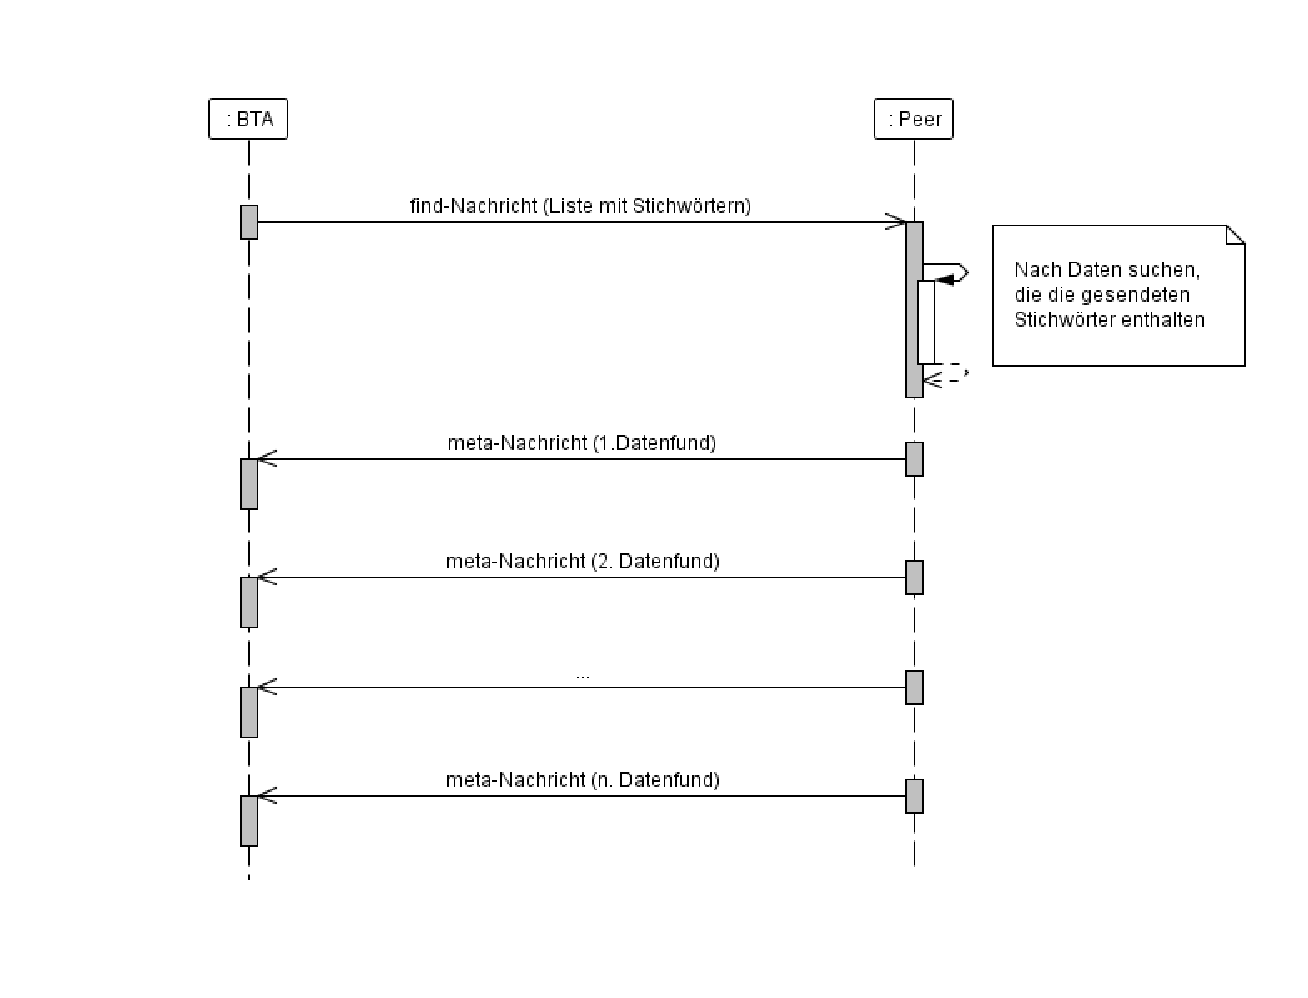
\includegraphics[width=\linewidth]{find.pdf}
	\caption{Beispiel für eine zulässige Suchanfrage}
\end{figure}

\begin{figure}[hpt]
	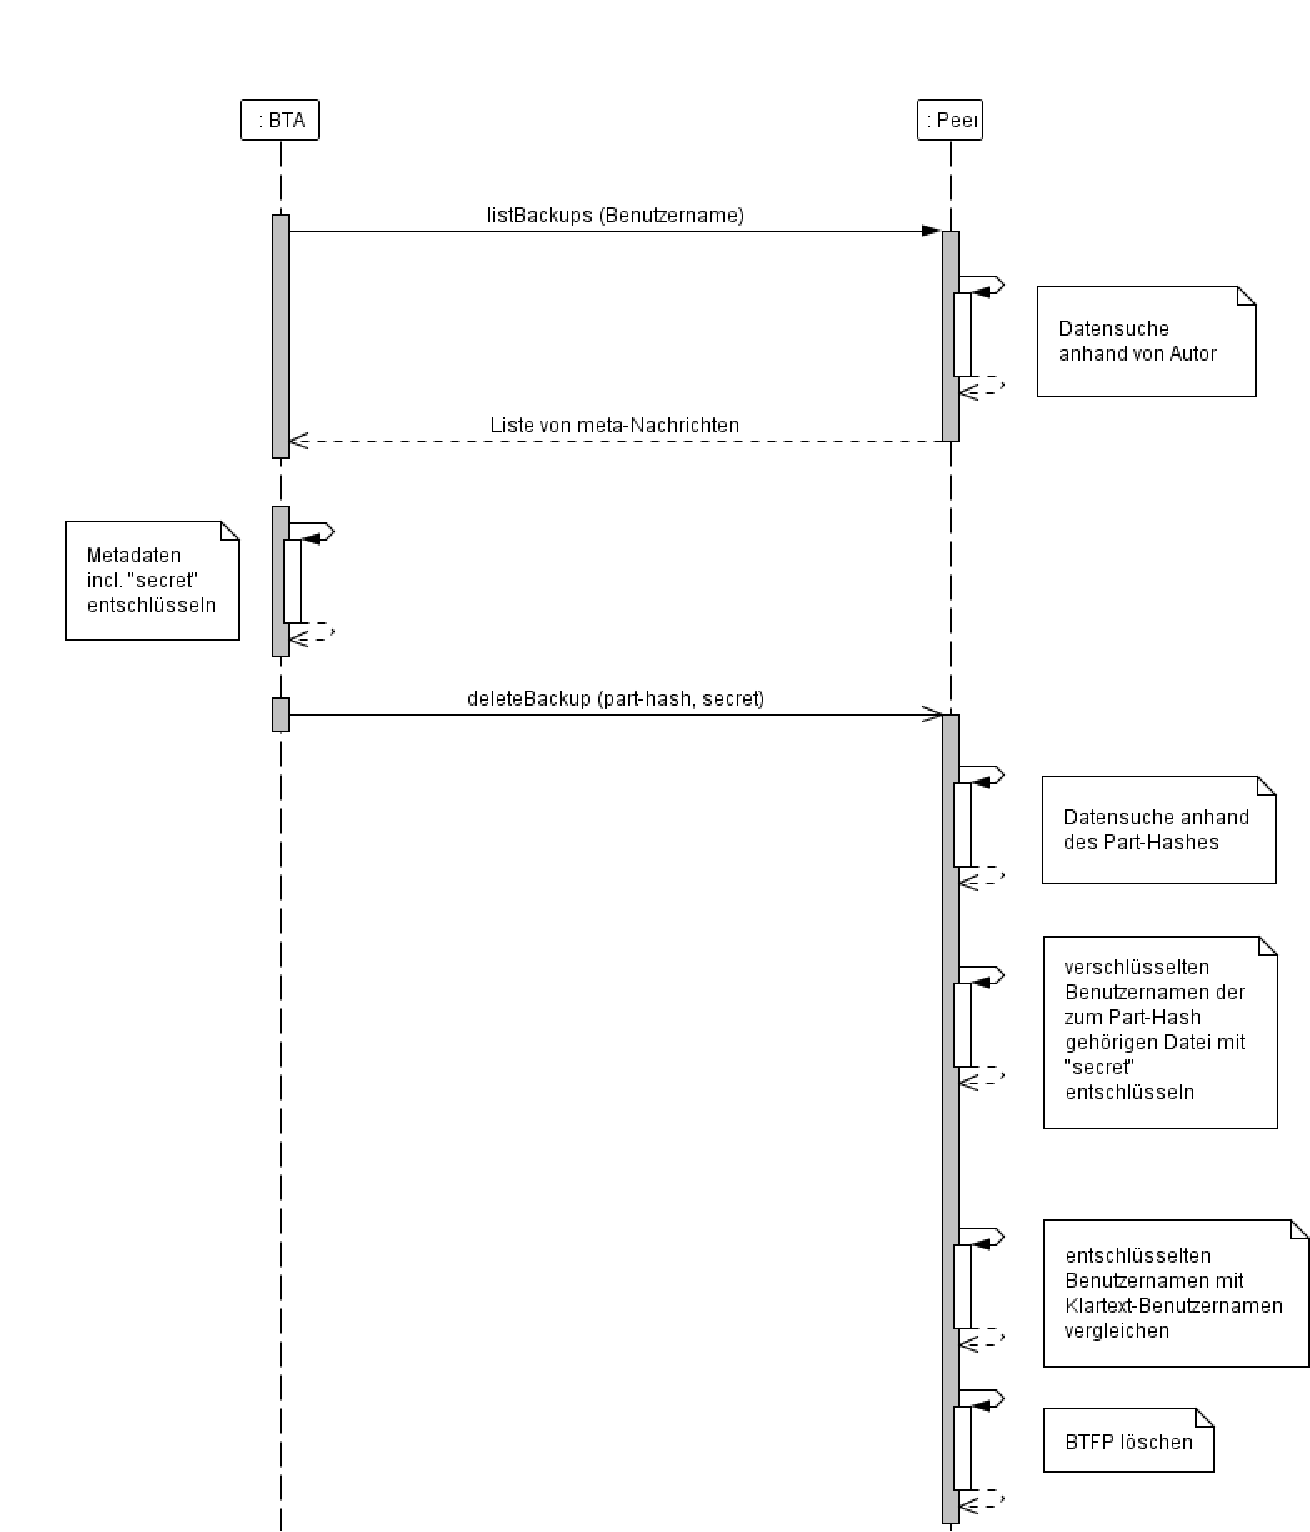
\includegraphics[width=\linewidth]{deleteBackup.pdf}
	\caption{Beispiel für eine zulässige Löschanfrage}
\end{figure}
